\documentclass[12pt, addpoints]{exam/exam}

\usepackage{hyperref}
%\usepackage{mdframed}
\usepackage{graphicx, caption}	
%\usepackage{array, multicol, tabu}
\usepackage{amsmath, amsthm, amssymb}
\usepackage{comment}
\usepackage{enumitem}
\usepackage{url}
\usepackage{textcomp}
\usepackage{wrapfig}
\newcommand{\1}{^{-1}}
\newcommand{\vect}[1]{\mathbf{#1}}
\newcommand{\R}{\mathbb R}
\newcommand{\vstr}{\vspace{\stretch{1}}}
\everymath{\displaystyle}
\setlength{\parindent}{0pt}

\theoremstyle{plain}
\newtheorem{thm}{Theorem}
\newtheorem*{thm*}{Theorem}

%\printanswers
\pointformat{\bf(\thepoints)}
\pointpoints{pt}{pts}
\bonuspointformat{\bf(\thepoints)}
\bonuspointpoints{pt}{pts}

\coverfirstpageheader{\bf MATH 235 (Calculus I) \\
		Fall 2017 \\
		}
		{}
		{{Name:} \underline{\hspace{40ex}} \\
		\vspace{0.5pc}
		Thurs 16 Nov 2017}
\coverextraheadheight[2pc]{0in}
\coverfirstpagefooter{}{}{\Large Good luck!}
\coverrunningheader{}
	{Exam 3: Graphing with derivatives}
	{}
\coverrunningheadrule	
\coverrunningfootrule
\coverrunningfooter{Calc I Fall 2017}{}{p. \thepage\ (of \numpages)}

\firstpageheader{}
	{Exam 3: Graphing with derivatives}
	{}
\firstpageheadrule
\firstpagefootrule
\firstpagefooter{Calc I Fall 2017}{}{p. \thepage\ (of \numpages)}

\runningheadrule
\runningheader{}
	{Exam 3: Graphing with derivatives}
	{}
\runningfootrule
\runningfooter{Calc I Fall 2017}{}{p. \thepage\ (of \numpages)}

\title{\vspace{-8pc}
\vfill{\Huge
	\bf Exam 3: Graphing with derivatives \\ 
	(\S3.10, 4.1-4.6)} 
	}
%\author{}
\date{}

% % % % % % % % % % % % % % % % % % % %
\begin{document}

\begin{coverpages}
\maketitle
\thispagestyle{headandfoot}
\vspace{-4pc}
{\bf Exam Instructions:} You have 75 minutes to complete this exam.  Justification is required for all problems.  Notation matters!  You will also be penalized for missing units and rounding errors.  
No electronic devices (phones, iDevices, computers, etc) except for a \textbf{basic scientific calculator}.  On story problems, round to two decimal places. 

\vspace{1pc}
If you finish early then you may leave, UNLESS there are less than 5 minutes of class left.  To prevent disruption, if you finish with less than 5 minutes of class remaining then please stay seated and quiet.

\begin{flushright}
%In addition, please provide the following data:

\vspace{0.3in}
%Drill Instructor: \underline{\hspace{40ex}}

\vspace{0.3in}
%Drill Time: \underline{\hspace{40ex}}
\end{flushright}

\vfill
\textbf{Your signature below indicates that you have read this page and agree to follow the Academic Honesty Policies of James Madison University.}  

\vspace{0.3in}
Signature: {\bf (1 pt)} \underline{\hspace{73ex}}

% % % % % % % % % %
\newpage
\vspace*{\fill}
\gradetable
%\textbf{Formulas you may need:}
%\vspace{-2pc}
%\begin{center}
%\vspace*{\fill}
%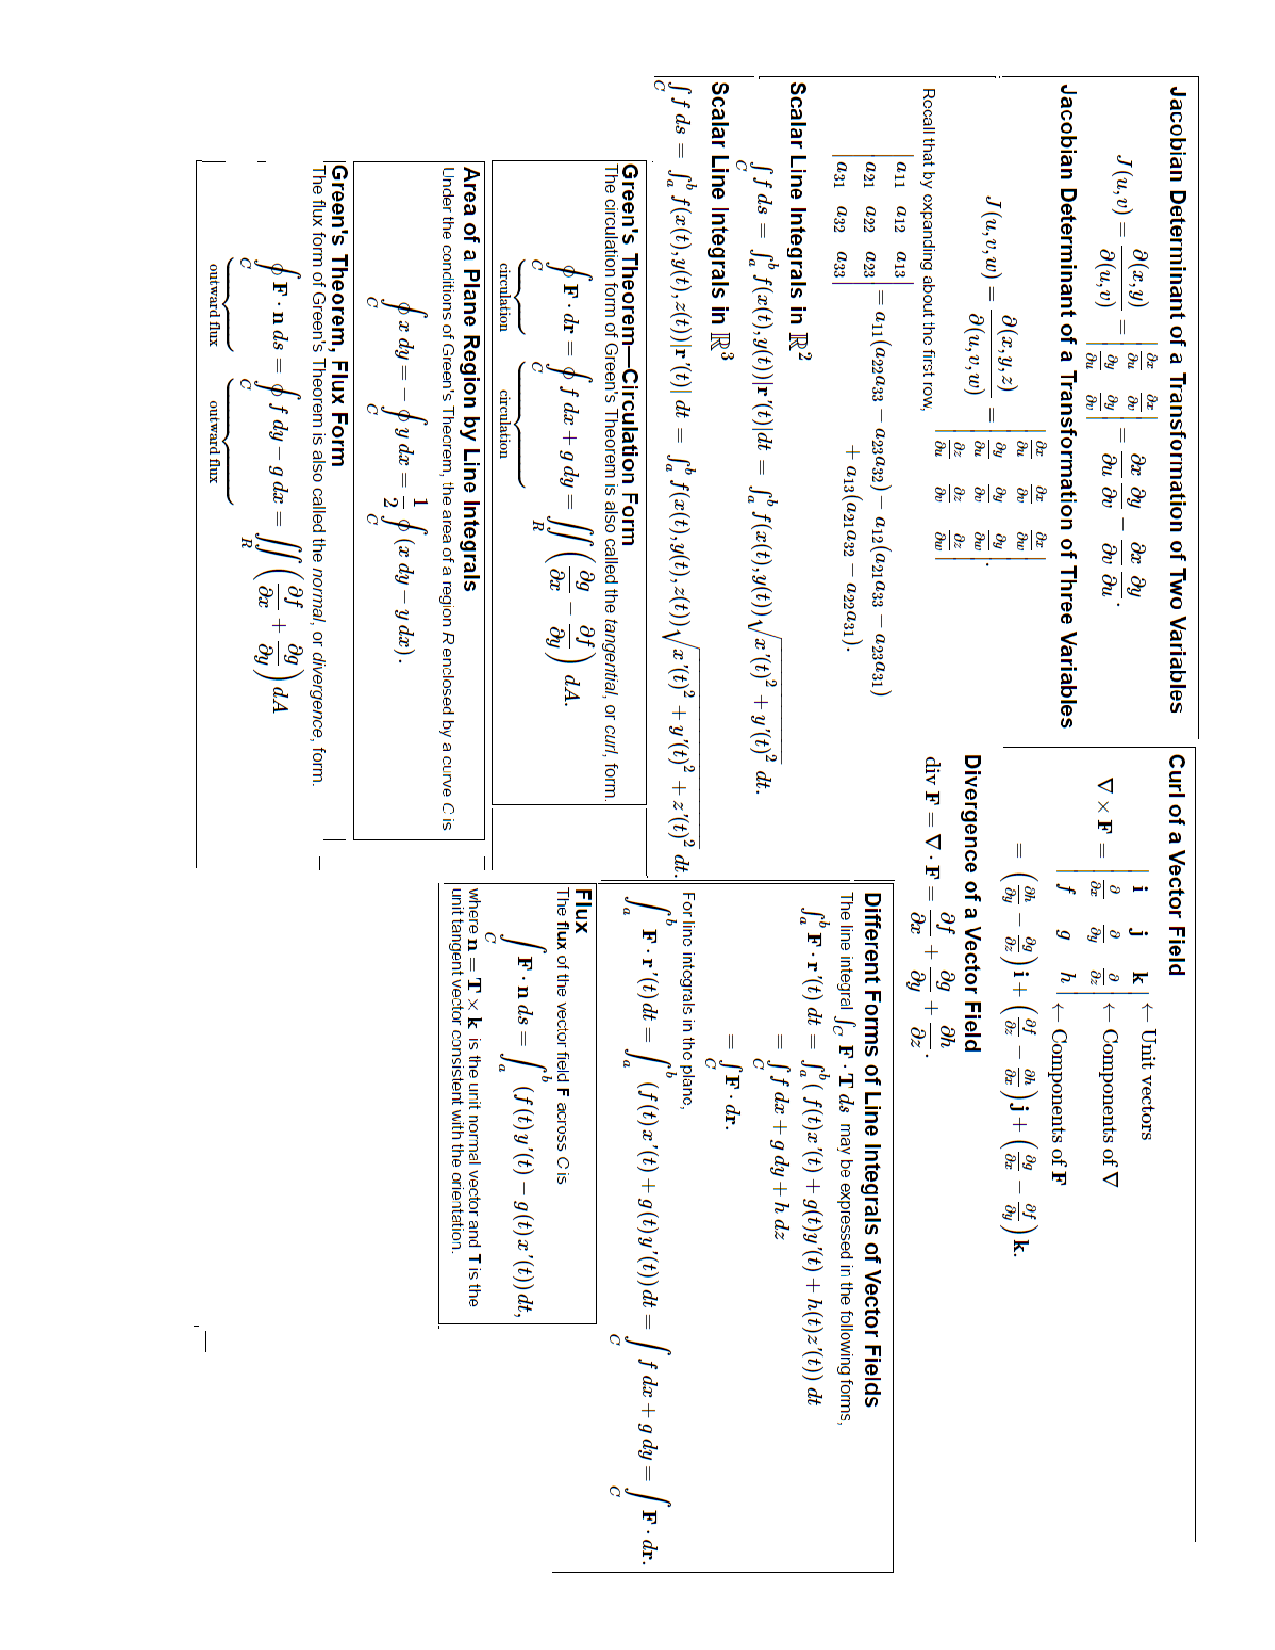
\includegraphics[scale=0.84]{Exam3FormulaSheet.pdf}
%\vspace*{\fill}
%\end{center}
\end{coverpages}

% % % % % % % % % % % % % % % % % % % %
\begin{questions}
\thispagestyle{headandfoot}

% % % % %
\question[] %{\bf 4.3 \#30} 
Sketch the graph of a function that satisfies all of the given conditions.
	\begin{itemize}
	\item $f'(0)=f'(4)=0$
	\item $f'(x)=1$ if $x<-1$
	\item $f'(x)>0$ if $0<x<2$
	\item $f'(x)<0$ if $-1<x<0$ or $2<x<4$ or $x>4$
	\item $\lim_{x\to 2^-}f'(x)=\infty$
	\item $\lim_{x\to 2^+}f'(x)=-\infty$
	\item $f''(x)>0$ if $-1<x<2$ or $2<x<4$
	\item $f''(x)<0$ if $x>4$
	\end{itemize}
	
%\newpage
% % % % %	
\question %{\bf 4.6 \#12} 
Let $f(x)=xe^{\frac{1}{x}}$.  Use the following steps to draw the graph of $f$ from scratch:
\vspace{0.5pc}
	\begin{parts}
	\part[] The behavior at $x=0$ is weird.  Use l'H\^opital's Rule to compute $\lim_{x\to 0^-}f(x)$ and $\lim_{x\to 0^+}f(x)$.
	%\vspace{30pc}
%	\vfill
	
%	\newpage
	\part[] What is the domain of $f$?
%	\vspace*{\fill}
	
	%\newpage
	\part[] Find the $x$- and $y$-intercepts.  If there are none, then say so.  If relevant, you may use information from part (a).
%	\vspace*{\fill}
	
	%\newpage
	\part[] Is $f$ even, odd, or neither?
%	\vspace*{\fill}
	
%	\newpage
	\part[] Determine the end behavior of $f$.  If relevant, you may use symmetry to save time.
	
%	\newpage
	\part[] Identify any vertical asymptotes.  If relevant, you may use information from part (a).
%	\vspace*{\fill}
	
	\part[] Find the critical points.
%	\vspace*{\fill}
	
	\part[] Use the 2nd Derivative Test to classify the critical points as local minima or maxima.  Identify which, if any, extrema are global.
%	\vspace*{\fill}
	
%	\newpage
	\part[] Identify intervals of increasing/decreasing.
%	\vspace*{\fill} 
	
	\part[] Identify intervals of concave up/down and points of inflection.
%	\vspace*{\fill}
	
	
%	\newpage
	\item Sketch the graph of $f$.  Your picture should be consistent with your answers to previous parts of the problem.
	\end{parts}

%\vfill

%\newpage
% % % % %
\question %{\bf 3.10 \#8}
 Let $f(x)=(1+x)^{-3}$.
	\begin{parts}
	\part[] Find the linearization of $f$ at $x=0$.
%	\vspace*{\fill}
	
	\part[] Find the differential $dy$.
%	\vspace*{\fill}
	
	\part[] Let $\Delta x=\frac{1}{3}$.  Find $\Delta y$ and $dy$.
%	\vspace*{\fill}
	
%	\newpage
	\part[] Sketch the graphs of $f$ and its linearization on the same axes.  \textit{Hint: To graph $f$, think about the graph of $\frac{1}{x^3}$.}  Label $dy$, $dx$, $\Delta y$, $\Delta x$, and $f(0)$.
	\end{parts}
	
\vfill	

%\newpage
% % % % %





\end{questions}

\end{document}